\chapter{How to ?}
\label{sec:faq}

\section{Introduction}
\label{faq:intro}

This section includes the FAQ avaible on \href{https://trac.feelpp.org/wiki/FAQ}{Feel web site}, if you want to post a question, please visit it and follow the instruction to edit the FAQ.
%This part is directly inspired by the same FAQ section on \href{\feel web site}{http://www.feelpp.org/files}

\section{Meshes}
\label{faq:meshes}

\subsection{What are the main execution options of a \feel application ?}
Let's consider that your application is named \lstinline!feelapp!, in that case you can modify the main execution options of your application with
\begin{unixcom}
		./feelapp --shape="simplex" --nochdir --exporter-format=gmsh
\end{unixcom}
These options are :
\begin{itemize}
\item \lstinline!shape=["simplex","hypercube"]! which is the shape of the generated mesh
\item \lstinline!nochdir! means that you want the result in the current directory (by default in \lstinline!~/feel!)
\item \lstinline!exporter-format! enables you to choose the format of mesh results output
\end{itemize}

\subsection{How to create a mesh?}
Here is an example of how to create a mesh with GMSH generator :

\begin{lstlisting}[language=sh]
 mesh_ptrtype mesh =
	createGMSHMesh( _mesh=new mesh_type,
         _update=MESH_CHECK!MESH_UPDATE_FACES!MESH_UPDATE_EDGES!MESH_RENUMBER,
         _desc=domain( _name= (boost::format( "%1%-%2%-%3%" ) %"hypercube" %Dim %1).str(),
         _shape="hypercube",
         _dim=Dim,
         _h=meshSize,
         _xmin=-1.,
         _xmax=1.,
         _ymin=-1.,
         _ymax=1. ) );
\end{lstlisting}

Here is an example of how to create a mesh with a .geo file :
\begin{lstlisting}[language=sh]
 mesh_ptrtype mesh =
	createGMSHMesh( _mesh=new mesh_type,
         _update=MESH_CHECK!MESH_UPDATE_FACES!MESH_UPDATE_EDGES!MESH_RENUMBER,
         _desc="???" );
\end{lstlisting}


\subsection{What are the different parameters of the function domain() ?}
The function \lstinline!domain()! is located in \lstinline!feel/feel/feefilters/gmsh.hpp! and enables to generate a simple geometrical domain from required and optional parameters. Its avaible options are :
\begin{itemize}
\item \lstinline!_name = "string"! gives the prefix of the gmsh geo and mesh files,
\item \lstinline!_shape = "simplex", "hypercube", "ellipsoid"! gives the shape of the domain, it is one of these three possibilities
\item \lstinline!_dim = 1, 2 or 3! gives the topological dimension of the domain. For example if \lstinline!_dim=2! and \lstinline!_shape="simplex"! this will produce a triangle
\item \lstinline!_h = real value! gives the characteristic size of the mesh, e.g. \lstinline!_h=0.1!
\item \lstinline!_xmin = real! gives the minimum x value of the domain for example \lstinline!_xmin=-1!
\item \lstinline!_xmax = real! gives the maximum x value of the domain for example \lstinline!_xmax=-1!
\item \lstinline!_ymin = real! gives the minimum x value of the domain for example \lstinline!_ymin=-1!.
\item \lstinline!_ymax = real!  gives the maximum y value of the domain for example \lstinline!_ymax=1!.

\end{itemize}


\subsection{How to loop on the degrees of freedom coordinates of a function ?}

Take a look at the example which is in \lstinline!feel/examples/snippets/dofpoints.cpp!

%\lstinputlisting[linerange=marker1-endmarker1]{../../..examples/snippets/dofpoints.cpp}

\subsection{How to work with specific meshes ?}
\label{howto:spec-meshes}
\marginpar{\lstinline!loadmesh.cpp!}
\feel supports several meshes file formats. It supports essentially Gmsh mesh file format but other are acceptable,  with some modifications :
\begin{itemize}

\item medit (\lstinline!.mesh!) \\
There is a small difference between medit meshes and gmsh ones. The medit reader of Gmsh is able to read medit meshes, the issue comes from markers for areas of the edges were we want to apply different boundary conditions. Gmsh is currently using the Physical Entities (physical line, area, volume). Unfortunetly, the medit reader of Gmsh considers the physical flag as null (to go deeper, you can check this part on \href{http://geuz.org/gmsh/doc/texinfo/gmsh.html#Elementary-vs-physical-entities}{Gmsh web site}). This option is took into account in \feel, the only modification is to put the optional parameter \lstinline!physical_are_elementary_regions! as \lstinline!true! in both functions \lstinline!createGMSHMesh! and/or \lstinline!loadGMSHMesh!. We have prepared a simple example which imports a \lstinline!medit! mesh with a surface and volume calculation on it. You can find it in \lstinline!feel/doc/manual/loadmesh.cpp!.

Please not that furthers \lstinline!medit! meshes are presented in example in the directory \lstinline!/feel/data/medit/!. The \lstinline!geo! scripts are those which are produced by \feel when reading those meshes.

\item Stl (\lstinline!.stl!) \\
You can also use \lstinline!stl! files, those files are native to the stereolithography CAD software created by 3D Systems. These files describe only the surface geometry of a three dimensional object without any representation of color, texture or other common attributes. You have further examples of such files in \lstinline!feel/data/stl!.

To use \feel with \lstinline!stl! files, you have to create a \lstinline!geo! script to enable gmsh to remesh the file. The \lstinline!stl! file you want to use has to be a volume mesh. The script is very small, you have all informations to make one at \href{https://geuz.org/trac/gmsh/wiki/STLRemeshing}{Gmsh/slt section} on their web site. Once it's done, you juste have to type
\begin{unixcom}
		gmsh stl_file_name.geo -3
\end{unixcom}
with \lstinline!stl_file_name.stl! in the same directory. That command will produce you the correct \lstinline!.msh! mesh that you could now use as usual without any modification in your \feel application.

 Take a look above how the remesh has produced a complete mesh with the file \lstinline!pelvis.stl! and \lstinline!pelvis.geo!:

\begin{figure}[!h]
\begin{minipage}[b]{.50\linewidth}
\centering
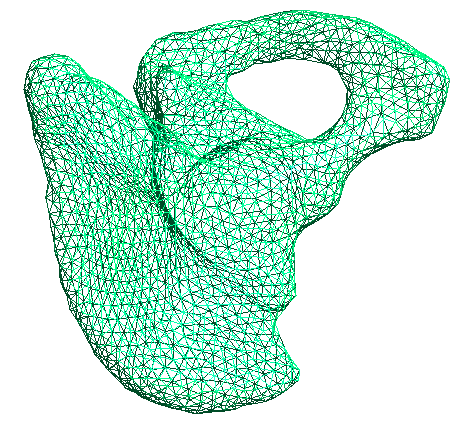
\includegraphics[width=4.5cm]{pngs/mymesh/pelvis_stl.png}
\caption{Pelvis before remesh (stl)}
\end{minipage}
\begin{minipage}[b]{.50\linewidth}
\centering
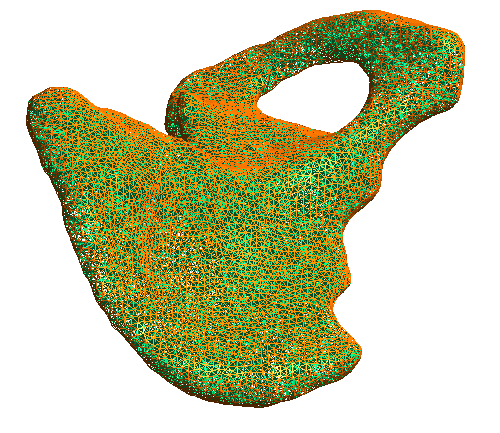
\includegraphics[width=4.5cm]{pngs/mymesh/pelvis_msh.png}
\caption{Pelvis after remesh (msh)}
\end{minipage}
\end{figure}

\end{itemize}


\section{Language for Partial Differential Equations}
\label{faq:PDE}

\subsection{What is the difference between using the "vf::project" function and solve a weak projection problem ?}

To make it clear, let's considerate that we want to project a $\mathbb{P}_1$ scalar function $\sigma$ on a $\mathbb{P}_0$ space. We have two alternatives to do it :
\begin{itemize}
\item Computing the $\mathcal{L}_2$ projection of $\sigma$ onto the space \newline
Here $kappa$ and $v$ are $\mathbb{P}_0$ functions :
\begin{lstlisting}
Matrix_M=integrate(elements(mesh), idt(kappa) * id(v));
Vector_F=integrate(elements(mesh), idv(sigma) * id(v));
\end{lstlisting}

\item Use the project function \lstinline!vf::project! \newline
This function does a nodal projection : at the dof point the projection will be \underline{exactly} equal to the projected function $\sigma$. It works as follow
\begin{lstlisting}
kappa=vf::project(P0_space, elements(mesh), idv(sigma));
\end{lstlisting}
\end{itemize}

These two projections are in general different, if you compare the values in the vector, they will be (slightly) different. However as $h \rightarrow 0$ they should both converge to the $\sigma$ function.


\subsection{How to do a quick L2 projection of an expression ?}
Let say that we have created two spaces, one scalar and one vectorial, we call them $\displaystyle{X_h}$ and $\displaystyle{X_{hVec}}$ and one wants to project some expressions on those spaces. \newline \newline
For example, we want to project $\displaystyle{(x,y) \rightarrow \sqrt{x^2 - y^2} -1}$ on the scalar space and $\displaystyle{(-2y, \cos{x})}$ on the vectorial space.
First of all, one has to create projectors for the scalar and vectorial spaces, the code reads as follow :
\begin{lstlisting}
#include <feel/feeldiscr/projector.hpp>
auto l2p = projector(Xh, Xh);
auto l2pVec = projector(XhVec, XhVec);
\end{lstlisting}
You can note that \lstinline!projector(Space, Space)! returns a \lstinline!boost::shared_ptr! on a \lstinline!Projector! object which makes projecting functions on \lstinline!Space! possible.
\newline \newline
Then, one uses the function \lstinline!Projector::project(Expression)! :
\begin{lstlisting}
auto Circle = l2p->project( sqrt( pow((vf::Px()),2.0)+ pow((vf::Py()),2.0)) - 1 );

auto F = l2pVec->project( -2 * Py() * oneX() + cos(vf::Px()) * oneY() );
\end{lstlisting}
Here you can note that the types of \lstinline!Circle! and \lstinline!F! are respectively : $X_{h}\_type::element\_type$ and $X_{hVec}\_type::element\_type$
\newline
An equivalent way to write it is to use the \lstinline!Projector::operator()(Expression)! :
\begin{lstlisting}
auto Circle = (*l2p)( sqrt( pow((vf::Px()),2.0)+ pow((vf::Py()),2.0)) - 1 );

auto F = (*l2pVec)( -2 * Py() * oneX() + cos(vf::Px()) * oneY() );
\end{lstlisting}
\lstinline!Projector::operator()! accepts many types of arguments, see \lstinline!feel/feeldiscr/projector.hpp! for details.



\subsection{How to compose \feel operators ?}

Let's considerate that we have created two spaces, one scalar $X_h$ and one vectorial $X_{hVec}$. We also have two vectors $a$ and $b$ (of type $X_{h}\_type::element\_type$).

One wants to do the following operation : $div( grad(a*b))$. The following expression is \textbf{not} yet implemented in \feel :
\begin{lstlisting}
divv( gradv( idv(a) * idv(b) ) )
\end{lstlisting}
One has to do intermediate projections to compose the operators. Using the Projector class, the code reads :
\begin{lstlisting}
#include <feel/feeldiscr/projector.hpp>

// create projectors on Xh and XhVec spaces
auto l2p = projector(Xh, Xh);
auto l2pVec = projector(XhVec, XhVec);

auto ab = l2p->project( idv(a)*idv(b) );
auto grad_ab = l2pVec->project( gradv(ab) );
auto div_grad_ab = l2p->project( divv(grad_ab) );
\end{lstlisting}
Here \lstinline!div_grad_ab! has the type $X_{h}\_type::element_type$. There is an equivalent but verboseless way to write this composition : use the \lstinline!Projector::operator()! which accepts has argument an expression or an \lstinline!element_type!. So one could write :
\begin{lstlisting}
#include <feel/feeldiscr/projector.hpp>

//create projectors on Xh and XhVec spaces
auto l2p = projector(Xh, Xh);
auto l2pVec = projector(XhVec, XhVec);

auto div_grad_ab = (*l2p)( divv( (*l2pVec)( gradv( (*l2p)(idv(a)*idv(b)) ) ) ) );
\end{lstlisting}
the * is needed before \lstinline!l2p! or \lstinline!l2pVec! since there are \lstinline!boost::shared_ptr! objects. One could also create directly \lstinline!Projector! objects :
\begin{lstlisting}
Projector<Xh_type, Xh_type> l2p(Xh, Xh);

auto ab = l2p(idv(a)*idv(b));
\end{lstlisting}


%%% Local Variables:
%%% coding: utf-8
%%% mode: latex
%%% TeX-PDF-mode: t
%%% TeX-parse-self: t
%%% x-symbol-8bits: nil
%%% TeX-auto-regexp-list: TeX-auto-full-regexp-list
%%% TeX-master: "feelpp-manual"
%%% ispell-local-dictionary: "american"
%%% End:

